

\begin{comment}
	\begin{frame}{Motivación}
		\dificultyLevel{1}
		\begin{itemize}[<+- | alert@+>]
			\item Para calcular ASV se requiere evaluar $\charactheristicFunction(\pi_{<i})$.
			\item Esto implica calcular esperanzas condicionales.
			\item Las redes bayesianas permiten representar distribuciones sobre los features.
			\item Necesitamos entender su estructura y cómo evaluar probabilidades en ellas.
		\end{itemize}
	\end{frame}
\end{comment}

\begin{frame}{Redes Bayesianas: Definición y Semántica}
\dificultyLevel{2}
\begin{mydefinition}
    Una red bayesiana $\aBayesianNetwork = (X, E, \Pr)$ consta de:
    \begin{itemize}
        \item Un DAG $(X,E)$: nodos son features, aristas son dependencias condicionales.
        \item Una función $Pr$ que codifica la probabilidad en base a esa red. %$Pr(x \mid \parents(x))$ para cada $x \in X$.
    \end{itemize}
\end{mydefinition}

\end{frame}

\begin{comment}
	\textbf{Probabilidad conjunta:}
	\[ Pr(X) = \prod_{x \in X} Pr(x \mid \parents(x)) \]
\end{comment}

\begin{frame}{Ejemplo: Red Bayesiana}
\dificultyLevel{2}
\begin{figure}
    \centering
    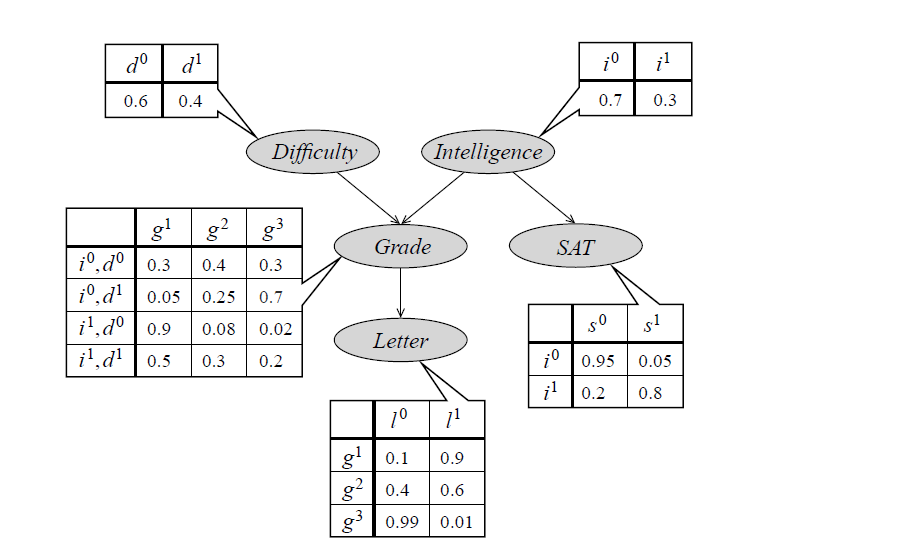
\includegraphics[scale=0.35]{pic/img/bayesianNetworks/bayesianNetworks.png}
    \caption*{Red bayesiana sobre datos de un estudiante con sus correspondientes Conditional Probability Tables (CPTs).  }%Fuente: \citet{probabilisticGraphicalModels}
\end{figure}
\end{frame}

\begin{frame}{Inferencia en Redes Bayesianas}
\dificultyLevel{2}
\begin{itemize}[<+- | alert@+>]
    \item \textbf{Inferencia}: calcular $Pr(C \mid E)$, la probabilidad del evento $C$ dada la evidencia $E$.
       
    \item El algoritmo que calcula la inferencia es \textit{Variable Elimination}.
    \item En polytrees es \textbf{polinomial}. En general es \#P-hard. Por lo tanto, vamos a utilizar redes bayesianas que sean \textbf{polytrees}. 
\end{itemize}
\end{frame}

\begin{comment}
	 \begin{itemize}
		\item $C$ va a ser la restricción que defina los valores que tiene la entidad. %, por ejemplo $\set{X_1 = 0, X_2=1, \dots}$
		\item $Evidence$ va a tener el mismo formato que $C$, pero va a ser la evidencia que tenemos respecto a los valores posibles de la entidad. 
	\end{itemize}
	
	\begin{frame}{Árboles de decisión y predicción promedio}
		\dificultyLevel{2}
		\begin{mydefinition}
			Un árbol de decisión $T$ es una estructura que evalúa instancias $e \in \entities(X)$ recorriendo nodos internos y asignando una salida en una hoja.
		\end{mydefinition}
		\pause
		\textbf{Objetivo:} calcular la predicción promedio del árbol condicionada en la evidencia. %, nuestra función $\charactheristicFunction(S)$. 
		%calcular el valor esperado $\mathbb{E}_{e \sim \Pr}[T(e)]$ condicionado a una evidencia.
	\end{frame}
\end{comment}



\begin{frame}{Árboles de decisión}
	\dificultyLevel{1}
	\begin{figure}
		\centering
		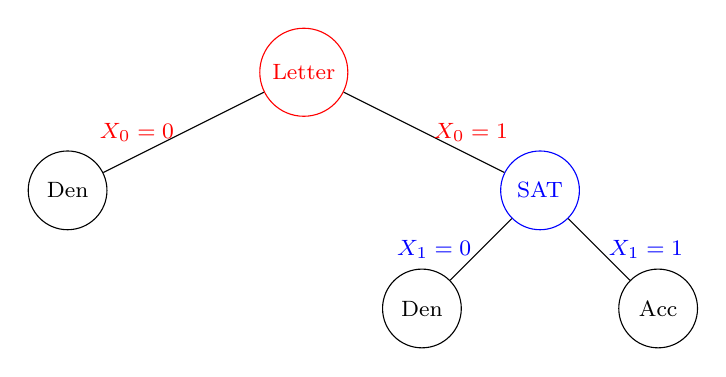
\begin{tikzpicture}[
			level 1/.style={sibling distance=6cm},
			level 2/.style={sibling distance=3cm},
			every node/.style={minimum size=1cm, font=\footnotesize}]
			\node [circle, draw, red] {Letter}
			child {
				node [circle, draw] {Den}
				edge from parent node[left] {\textcolor{red}{$X_0 = 0$}}
			}
			child {
				node [circle, draw, blue] {SAT}
				child {
					node [circle, draw] {Den}
					edge from parent node[left] {\textcolor{blue}{$X_1 = 0$}}
				}
				child {
					node [circle, draw] {Acc}
					edge from parent node[right] {\textcolor{blue}{$X_1 = 1$}}
				}
				edge from parent node[right] {\textcolor{red}{$X_0 = 1$}}
			};
		\end{tikzpicture}
		\caption*{Árbol de decisión que define si un estudiante va a ser aceptado (accepted/1) o rechazado (denied/0) en su ingreso a una universidad.}
	\end{figure}
	\pause
	\textbf{Objetivo:} calcular la predicción promedio del árbol condicionada en la evidencia. %, nuestra función $\charactheristicFunction(S)$.
\end{frame}


\begin{comment}
	\begin{frame}{Supuestos del Algoritmo}
		\dificultyLevel{3}
		\begin{itemize}[<+- | alert@+>]
			\item Para este algoritmo trabajaremos con:
			\begin{itemize}
				\item Árboles de decisión \emph{binarios}.
				\item Features \emph{binarios}.
			\end{itemize}
			\item Más adelante veremos la extensión a variables no binarias.
			\item Definimos dos conjuntos de asignaciones sobre features:
			\begin{itemize}
				\item \(\;ev\): evidencia conocida. %(conjunto de asignaciones \(X_i = k\) fija).
				\item \(\;pathCondition\): condiciones acumuladas durante el recorrido. % (también un conjunto de asignaciones \(X_i = k\)).
			\end{itemize}
		\end{itemize}
	\end{frame}
	
	\item Cada nodo del árbol determina un valor para un feature \(X_i\):
	\begin{itemize}
		\item Hijo izquierdo \(\Rightarrow X_i = 0\).
		\item Hijo derecho   \(\Rightarrow X_i = 1\).
	\end{itemize}
	
	\begin{itemize}
		\item En cada nodo, agregar la asignación correspondiente a \(\,pathCondition\) según cada rama.
	\end{itemize}
\end{comment}

\begin{comment}
	\begin{frame}{Algoritmo de promedio}
		\dificultyLevel{3}
		\begin{enumerate}[<+- | alert@+>]
			\item Recorrer todas las ramas del árbol de decisión, acumulando las decisiones tomadas.
			\item Al llegar a una hoja:
			\begin{itemize}
				\item Evaluar la probabilidad de haber alcanzado esa hoja, dada la evidencia. 
				%\[ Pr_B\bigl(pathCondition \mid ev\bigr).\]
				\item Luego multiplicar dicha probabilidad por el valor de salida que retorna la hoja.
			\end{itemize}
			\item Sumar todas las contribuciones de cada hoja para obtener la predicción promedio. 
		\end{enumerate}
	\end{frame}
	
	\begin{frame}[fragile]{Algoritmo: Predicción Promedio}
		\dificultyLevel{3}
		\begin{algorithm}[H] % ← evita que flote
			\caption{Predicción promedio para árbol de decisión binario}
			\footnotesize            % opcional: letra más chica
			\begin{algorithmic}[1]
				\Function{Mean}{$node$, $B$, $pathCondition$, $evidence$}
				\If{$evidence$ no coincide con $pathCondition$}
				\State \Return $0$
				\EndIf
				\If{$node$.isLeaf}
				\State \Return $Pr_B(pathCondition \mid evidence)\cdot node.value$
				\EndIf
				\State $X_i \gets node.feature$
				\State $left \gets$  \Call{Mean}{$node$.left,  $B$, $pathCondition \cup\{X_i=0\}, evidence$}
				\State $right\gets$  \Call{Mean}{$node$.right, $B$, $pathCondition \cup\{X_i=1\}, evidence$}
				\State \Return $left + right$
				\EndFunction
			\end{algorithmic}
		\end{algorithm}
		\vspace{0.3cm}
		Complejidad: $O(i|V| + l \cdot varElim)$, polinomial si $varElim$ lo es (e.g. polytrees).
	\end{frame}
	
	\begin{frame}{Extensión a Features No Binarios}
		\dificultyLevel{2}
		\begin{itemize}[<+- | alert@+>]
			\item El algoritmo original funciona con árboles y variables \textbf{binarios}.
			\item Para admitir \textbf{features no binarios} adaptamos la inferencia.
			\item Al llegar a un nodo con umbral \(v\), dividimos el dominio de \(f\):
			\begin{itemize}
				\item Lado izquierdo: \(f = i\) con \(i < v\)
				\item Lado derecho: \(f = d\) con \(d \geq v\)
			\end{itemize}
			\item La probabilidad condicional requiere una \textbf{suma de múltiples consultas}. 
			\begin{itemize}
				\item  Si tuviéramos la consulta \set{$X_1 \in \set{1,2}, X_2 = 3$} la resolvemos cómo:
				\[
				Pr_B(X_1=1, X_2=3) + Pr_B(X_1=2, X_2=3)
				\]
			\end{itemize}
			\item Esto hace que la complejidad ya no sea polinomial.
			\item No optimizamos esta inferencia, ya que excede los objetivos de la tesis.
		\end{itemize}
	\end{frame}

	\begin{frame}{Cálculo Ejemplo}
		\dificultyLevel{2}
		\scriptsize
		\begin{align*}
			&\Call{Mean}{Letter,\,B,\,\{\},\,\{INT = 1\}}\\
			&= \; \underbrace{\Call{Mean}{Den,\,B,\,\color{red}{\{Letter = 0\}},\,\color{brown}{\{INT = 1\}}}}_{=0} 
			\;+\; \Call{Mean}{SAT,\,B,\,\color{red}{\{Letter = 1\}},\,\color{brown}{\{INT = 1\}}} \\[0.5em]
			&= 0 \;+\; \Call{Mean}{SAT,\,B,\,\{Letter = 1\},\,\{INT = 1\}}\\[0.5em]
			&= \; \Call{Mean}{Den,\,B,\,\{Letter = 1,\;\color{red}{SAT = 0}\},\,\{INT = 1\}} 
			\;+\; \Call{Mean}{Acc,\,B,\, \dots)}\\[0.5em]
			&= \; Pr_{B}\bigl(SAT = 0,\,Letter = 1 \mid INT = 1\bigr)\;\cdot 0 
			\;+\; Pr_{B}\bigl(SAT = 1,\,Letter = 1 \mid INT = 1\bigr)\;\cdot 1\\[0.5em]
			&= \; Pr_{B}\bigl(SAT = 1,\,Letter = 1 \mid INT = 1\bigr)\\
			&= 0.61
		\end{align*}
		\textbf{Nota:} la evidencia afecta la predicción aún si el feature no aparece en el árbol.
	\end{frame}
\end{comment}

